Una vez definido el algoritmo, se va a explicar la implementación que se ha llevado a cabo teniendo en cuenta las ventajas y limitaciones de la arquitectura. En este caso, orientar el diseño a una FPGA va a condicionar en gran medida la toma de decisiones en este aspecto. 

\begin{figure}[!ht]
\begin{center}
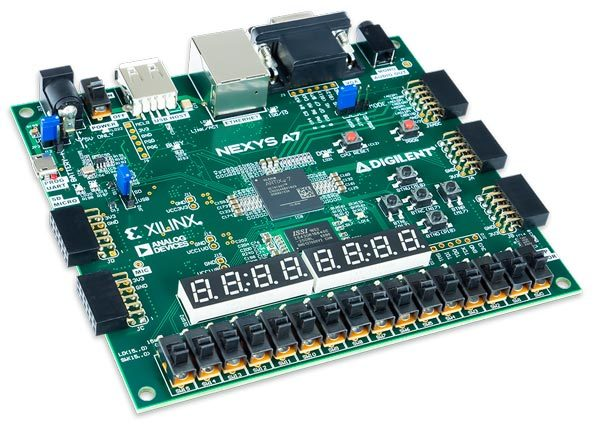
\includegraphics[width=10cm]{img/nexysa7.jpg}
\caption{\label{fig:nexys}Placa Nexys A7}
\end{center}
\end{figure}

Para el montaje de prototipo, se va a utilizar la placa proporcionada por el departamento: Nexys A7 de Digilent, mostrada en la figura \ref{fig:nexys}. Esta placa monta una FPGA de la familia Artix-7 modelo \emph{XC7A100T-1CSG324C} junto con múltiples añadidos para conectividad, entrada y salida de datos, sensor de temperatura y acelerómetro. Además incluye varios diodos LED, que junto a los botones y conmutadores, permiten un cómodo manejo del conjunto de la placa. El conjunto de las prestaciones será más que suficiente para probar más adelante el funcionamiento del prototipo.

De especial trascendencia para la puesta en marcha del conjunto, serán las bahías de pines que se ubican en ambos laterales de la Nexys, puesto que permiten conectar y leer los voltajes de entrada y salida de las señales que se utilizarán. La documentación proporcionada por Digilent \cite{Nexys} ha resultado muchas veces insuficiente, pero fundamental a la hora de poner en marcha el prototipo.

\section{Gestión entrada-salida}
Siguiendo el flujo de datos desde la etapa analógica, el primer paso consiste en introducir los mismos en la FPGA. Para ello, es imprescindible convertir el voltaje analógico en la señal digital mediante el uso de un \emph{Conversor Analógico a Digital}, en lo sucesivo ADC. La Nexys A7 no incorpora ninguno integrado por lo que habrá que conectarlo externamente. Adelantando los acontecimientos, será necesario también un \emph{Conversor Digital a Analógico}, o DAC, para reconvertir a tensión analógica la salida de audio procesado. Por ello, se decide buscar ambos conversores conjuntamente, para simplificar su puesta en marcha.

Existen infinidad de conversores de este tipo en el mercado, todos ellos ideados para operar en diferentes condiciones de trabajo, en diferentes formatos y a un precio muy asequible. En el caso de las señales de audio, la mayor especificación que deben de cumplir es el compromiso de la tasa de muestreo $t_{s}$ (o más frecuentemente su inversa, la \emph{frecuencia de muestreo} $F_{s}$) para no corromper la señal entrante y preservar su calidad. Típica mente se utilizan algunos valores ya estandarizados por las grandes compañías de audio a lo largo del siglo XX:

\begin{itemize}
\item \textbf{$F_{s} = 8kHz$:} Utilizada especialmente para telefonía comercial pero no para componentes de audio de carácter musical.
\item \textbf{$F_{s} = 22050Hz$:} Frecuencia de muestreo típica de la radio que permite reproducir señales con componentes máximas de hasta 10kHz.
\item \textbf{$F_{s} = 32kHz$:} Se utiliza no tan frecuentemente en varios formatos de vídeo digital, como el miniDV.
\item \textbf{$F_{s} = 44,1kHz$:} La más extendida en formatos como MP3, MPEG y CD por razones tanto históricas como prácticas. Puesto que un oído joven es capaz de percibir tonos de hasta 20kHz aproximadamente, esta tasa se estableció tras aplicar el criterio de Nyquist dejando un margen suficiente para compensar las etapas de filtrado posteriores.
\item \textbf{$F_{s} = 48kHz$:} También muy utilizada en televisión digital, DVD y audio profesional.
\item \textbf{$F_{s} = 96 o 192,4kHz$:} Pensada especialmente para audio de alta definición en formatos como HD-DVD y Blue-Ray Disc
\end{itemize}

Tras analizar las posibilidades, resulta evidente que para una aplicación de audio musical conviene establecer la frecuencia de muestro en 44,1 o 48 kHz de forma que conserve cierta similitud con los equipos comerciales y profesionales del mercado.

Así, aprovechando su reciente adquisición por parte del departamento, se va utilizar un componente que integre tanto ADC como DAC y que permita trabajar a estas velocidades: el \emph{Pmod i2s2} también de Digilent.

\subsection{Pmod i2s2}
Este componente trae, en definitiva todo lo necesario para este proyecto: junto a los ADC y DAC incorpora dos puertos para mini-jack estéreo hembra\footnote{Lo más extendido para audio, puesto que son los conectores que llevan móviles, auriculares. ordenadores, etc...} y una serie de pines dispuestos de tal forma que la conexión con la placa es inmediata. Se pueden observar estas características en la imagen \ref{fig:pmod}.

\begin{figure}[!ht]
\begin{center}
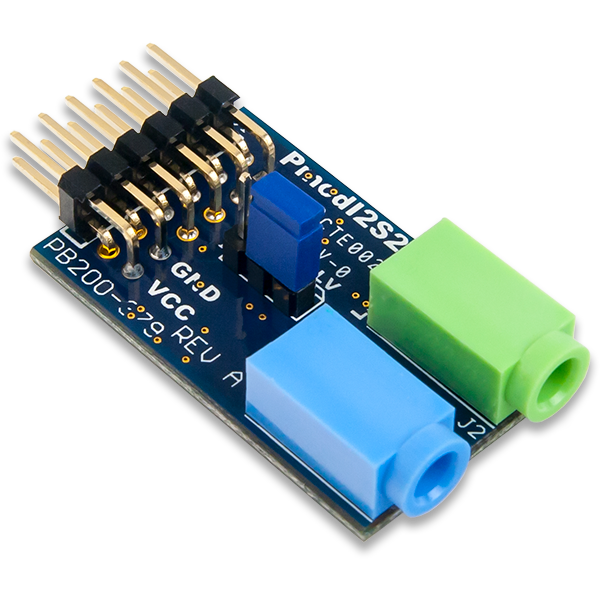
\includegraphics[width=6cm]{img/pmod.png}
\caption{\label{fig:pmod}Detalle del Pmod i2s2}
\end{center}
\end{figure}

Lógicamente, al ser ambos placa y \emph{plug-in} fabricados por Digilent, no hay ningún problema para conectarlos entre sí, basta con conectarlo a una de las bahías de pines que tiene la FPGA. Además, las conexiones de alimentación, Vcc y GND, se encuentran hechas de serie en la Nexys, por lo que no es necesario añadirlas en el fichero de conexiones o \emph{constraints}.

Tanto el modelo de ADC, \emph{Cirrus CS5345} \cite{adcdata}, como el de DAC, \emph{Cirrus CS4344} \cite{dacdata} realizan las conversiones con hasta 24 bit por muestra e incorporan un filtro paso bajo anti-aliasing que por tanto, no hará falta implementar. [EXPLICAR EL ALIASING?] Además tienen 98 dB de rango dinámico y baja distorsión armónica, haciéndolos ideales para las aplicaciones de audio, aún más cuando están conectados a entradas de \emph{mini-jack}.

Aunque los conversores soportan hasta 24 bit el tamaño de cada palabra serán 16 bit, debido a que es la longitud que utiliza el formato CD, con el que se intentará tener el mayor número de similitudes posibles. La otra diferencia de este formato será que el procesado será \emph{mono} en lugar de \emph{estéreo}. Evidentemente, la existencia de dos canales dobla el número de operaciones y la complejidad del algoritmo al tener que duplicar el flujo de datos en todos los puntos del diseño. Por ello, no se suelen utilizar conexiones ni procesados estéreo en instrumentos monofónicos\footnote{Instrumentos que solo pueden producir una nota al mismo tiempo} ya que estos suelen tener un lugar fijo en la imagen estéreo de la producción, siendo irrelevante su salida estéreo. En la práctica, se muestrearán los datos del canal izquierdo, que por convenio es el principal cuando solo se va a operar con un canal, y tras el procesado, se escribirá el resultado en ambos canales.

\subsection{Consideraciones de la implementación del Pmod}
La primera consideración que tuve que hacer trabajando con estos componentes fue \textbf{desconfiar totalmente de la guía de Digilent}. Esta compañía en lugar de proporcionar la información de sus productos en un único documento o \emph{datasheet}, tiene varias webs enlazadas con diversos documentos y enlaces a referencias de terceros que difícilmente facilitan el uso de los aparatos. Por tanto, se debe siempre recurrir a la documentación del fabricante: \emph{Cirrus Logic} en el caso de los conversores, \emph{Artix} en el caso de la FPGA, etc. Para llegar a esta conclusión he tenido que desperdiciar muchas horas contrastando la información entre diferentes fuentes que deberían ser idénticas.

En primer lugar es necesario conectar el Pmod con la placa, para ello basta insertarlo en la bahía de pines y modificar el archivo de conexiones \emph{.xdc}. Este archivo debe buscarse en la página de la Nexys A7, ya que en algunos ejemplos de Digilent en GitHub el numerado de los pines es incorrecto. Hay que recordar que estos archivos de conexiones tienen un lenguaje \emph{case sensitive}, distinguen entre minúsculas y mayúsculas, a diferencia del VHDL. En este tipo de ficheros tampoco puede haber dos señales con el mismo nombre, si es necesario duplicar una señal (que será obligatorio en varias señales como los relojes) debe hacerse desde el código principal VHDL y nombrarlo diferente de cara a las conexiones. 

\begin{figure}[!ht]
\begin{center}
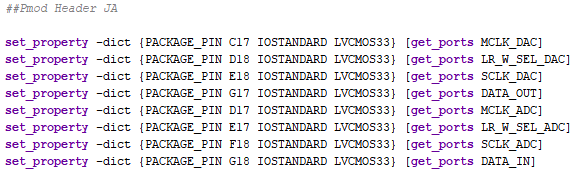
\includegraphics[width=12cm]{img/xdc.png}
\caption{\label{fig:xdc}Conexiones del Pmod con la FPGA en el fichero .xdc}
\end{center}
\end{figure}

La comunicación entre ambos módulos sigue un protocolo $I^{2}S$ \cite{i2s} el cual está bastante extendido en este tipo de aplicaciones con conversores y controladores. Este protocolo separa la señal de datos del resto de señales de control que son tres relojes (en este caso), de forma que se garantiza su funcionamiento síncrono. Estos relojes se generan en la FPGA que actúa de controlador maestro mientras que tanto el ADC como el DAC funcionan como esclavos. Se describen a continuación:

\begin{itemize}
\item \textbf{MCLK:} Es el reloj maestro del sistema a partir del cual se van a generar el resto. Su correcta generación resulta fundamental a la hora de mantener una correcta temporización, como se verá más adelante.
\item \textbf{SCLK:} Corresponde al reloj de bit, es decir, cada periodo de este corresponde a la duración del bit que va a ser leído. Una peculiaridad importante es que debe estar en contrafase con el resto de relojes.
\item \textbf{LRCK:} Representa la longitud de la palabra de cada canal, es decir, LRCK = 1 corresponde al canal derecho y LRCK = 0 al izquierdo, de forma que su lectura es alterna. Además es el reloj que representa la frecuencia de muestro ya que las palabras se suceden en intervalos de su propio periodo. En el proyecto de Vivado, se renombra a LR\_W\_SEL.
\end{itemize}


Es fundamental entender que las relaciones entre estos tres relojes aseguran tanto la correcta interpretación de los datos y su reconstrucción como la comunicación con el módulo maestro, es decir, la FPGA. Para este proyecto se ha fijado una frecuencia de \textbf{50~MHz} para el reloj maestro, ya que de esta forma es más sencilla su relación con el reloj de sistema de 100~MHz. Consultando la tabla de equivalencias proporcionada por el fabricante, imagen \ref{fig:flujoreloj}, podemos establecer la relación entre los relojes mediante divisiones por múltiplos de 2.

\begin{figure}[!b]
\begin{center}
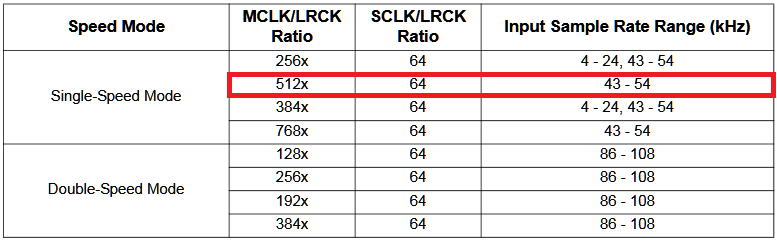
\includegraphics[width=15cm]{img/ratiosreloj.png}
\caption{\label{fig:flujoreloj}Tabla de las relaciones entre los relojes}
\end{center}
\end{figure}

\begin{figure}[!b]
\begin{center}
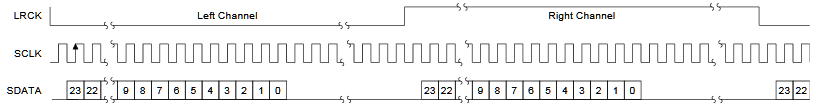
\includegraphics[width=14cm]{img/i2sov.png}
\caption{\label{fig:i2sov}Funcionamiento de los relojes de control con flujo de datos}
\end{center}
\end{figure}

Como la frecuencia de MCLK es fija dada por el sistema, para obtener la frecuencia de muestreo deseada en torno a los 44,1~kHz, hay que aplicar el factor 512. De esta forma si $F_{MCLK}~=~50~MHz$ entonces $F_{LRCK}~=~F_{MCLK}/512 = 97.656,25~Hz$ pero como esa frecuencia se comparte entre los dos canales, la frecuencia de muestreo final $F_{s}$ de un único canal resulta $F_{s} = 97.656,25/2 = 48.828,125 Hz \approx 48,8 kHz$. Finalmente, como el factor $F_{SCLK}/F_{LRCK}=64$ obtenemos $F_{SCLK}~=~3,135~MHz$. Como se puede ver, la frecuencia de muestreo obtenida es mayor de la buscada y necesaria, pero también guarda relación con el estándar de alta calidad, por lo que tampoco conviene cambiarla. Tener una relación inmediata con el reloj de sistema resulta muy conveniente.

Para generar estas frecuencias se barajó la opción de utilizar el \emph{clocking wizard}, un módulo IP de Vivado que garantiza la correcta relación entre una frecuencia entrante y cualesquiera que se configuraran salientes. Sin embargo, este solo admite frecuencias de salida en el rango de las decenas de megahercios. Por ello se ha tenido que implementar un contador que permitiera dividir la frecuencia en múltiplos de 2 usando los bit de esa señal. El pseudocódigo se muestra en la figura \ref{fig:controlsig}.

\begin{figure}[!h]
\begin{center}
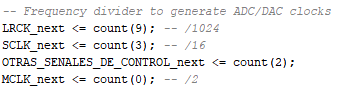
\includegraphics[width=7cm]{img/controlsig.png}
\caption{\label{fig:controlsig}Esquema de la generación de los relojes}
\end{center}
\end{figure}

Por último, la adquisición de los datos se realiza utilizando un registro de desplazamiento estándar propuesto por P.Chu \cite{vhdlchu}. Teniendo en cuenta que el primer dato, que será el bit más significativo o MSB, espera un ciclo de reloj antes de ser válido, tal y como se muestra en la figura \ref{fig:i2sov}. Como solo se van a procesar 16 bit, el resto de datos se ignoran hasta el siguiente ciclo.

\section{Controlador de datos}

El controlador que gestiona el flujo de entrada/salida de los datos es el llamado \emph{master\_controller}. Este se encarga de generar las señales necesarias para el correcto funcionamiento de Pmod y de instanciar el resto de componentes que utilizarán, a excepción de los displays. Para garantizar el flujo de datos apropiado, se modela mediante una máquina de estados, cuyo esquema corresponde a la figura \ref{fig:estados}. La lógica del cambio de estados está en un fichero aparte llamada \emph{fsm\-control}.

\begin{figure}[!th]
\begin{center}
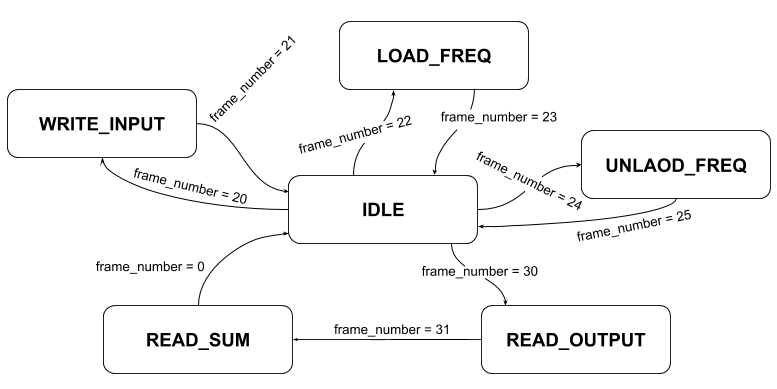
\includegraphics[width=13cm]{img/destados.png}
\caption{\label{fig:estados}Diagrama de estados del controlador de datos}
\end{center}
\end{figure}

Nótese que todos los cambios de estado los produce la variable \emph{frame\_number}, la cual se encarga de llevar la cuenta de los ciclos de reloj de bit (SCLK) que se producen en cada flanco del reloj de canal (LRCK) hasta un total de 32. Cada estado tiene una función concreta: 
\begin{itemize}
\item \textbf{IDLE:} Es el estado fundamental. Durante los 20 primeros ciclos se está produciendo la lectura de los datos de entrada y almacenándolo en un búfer, ya que el registro de desplazamiento se activa siempre en el mismo momento independientemente del estado, aunque este siempre vaya a ser IDLE.
\item \textbf{WRITE\_INPUT:} Lee el búfer donde está escrito el dato de entrada proveniente del ADC, le aplica el factor de enventanado que le corresponda y lo almacena en memoria.
\item \textbf{LOAD\_FREQ:} Traslada el dato de la memoria donde estaba almacenado al módulo que realiza la FFT. Como la velocidad de procesado es mucho más rápida que la frecuencia de muestreo, se evitarán las colisiones.
\item \textbf{UNLOAD\_FREQ:} Devuelve el dato procesado proveniente del módulo que realiza la iFFT y lo almacena en una memoria de salida.
\item \textbf{READ\_OUTPUT:} Lee los cuatro datos de las memorias de salida y los almacena un sus correspondientes registros.
\item \textbf{READ\_SUM:} Aplica la ventana de salida a las cuatro muestras ubicadas en los registros y las suma entre sí para obtener el dato que se va a escribir en el siguiente ciclo, el cuál se guarda nuevamente en un registro.
\end{itemize}

Salta a la vista que son necesarios varios bancos de memoria, cada uno ubicado en un punto diferente del flujo de datos. La implementación de cada uno de ello varía en función de su propósito, como se verá a continuación en \ref{memo}. Sin embargo, conviene primero aclarar cómo se lleva a cabo el proceso de enventanado, ya que condiciona en gran medida el diseño del flujo de datos.

\subsection{Implementación del solapamiento}
Como se ha descrito anteriormente, el factor de solapamiento que se va utilizar es del 75\%. Esto quiere decir que serán necesarias al menos cuatro memorias para poder almacenar toda la información, tal y como se muestra en la figura \ref{fig:solap}. 

\begin{figure}[!b]
\begin{center}
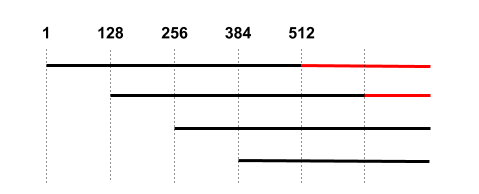
\includegraphics[width=13cm]{img/solap.png}
\caption{\label{fig:solap}Esquema del solapamiento entre las memorias}
\end{center}
\end{figure}

Cada una de las barras horizontales representa a una de las cuatro ventanas. Es importante asegurar que la muestra entrante se multiplica por el coeficiente de enventanado adecuado, que depende exclusivamente de la posición de la muestra en la ventana. De esta forma, la palabra entrante se registra una vez para luego ser multiplicada por la constante de cada ventana antes de ser almacenada en su memoria correspondiente.

En el momento de la reconstrucción, es necesario hacer cuatro accesos a memoria que recuperen cada uno de los cuatro datos procesados para multiplicar nuevamente por la constante apropiada y sumarlos todos entre sí. Los valores de las constantes de ambas ventanas garantizan que no haya desbordamiento en esta suma.

Los coeficientes de enventanado que se utilizan durante el procesado se almacenan en dos memorias no volátiles, una para cada ventana. Estas memorias se generan utilizando únicamente lógica combinacional en VHDL, para minimizar la latencia de las mismas. Para no introduir todos los valores de forma manual, se han generado los fichos VHDL mediante un script de Matlab ubicado en el Apéndice \ref{ap:script}

\subsection{Bancos de memorias\label{memo}}
Todas las memorias volátiles del proyecto están implementadas utilizando los módulos de Vivado \emph{Block Memory Generator}. Estos asistentes permiten crear memorias RAM y ROM si fuesen necesarias e inicializar cualquiera de ellas a un valor determinado usando un fichero de texto. En este caso se han utilizado dos de estos tipos dependiendo de su funcionalidad en el proyecto.

En el caso de las memorias de entrada, está garantizado que no existan colisiones de ningún tipo en el proceso de lectura y en el de escritura, por lo que se puede utilizar el diseño más simple que propone Vivado, las memorias RAM de puerto único \cite{ram}, ubicada a la derecha en la figura \ref{fig:rams}. Este tipo de memorias poseen un puerto llamado \emph{WEA} que conmuta la posición de lectura y escritura. Su uso está destinado a los bloques en los que este garantizado que no existan estas colisiones, como por ejemplo en la adquisición de los datos de entrada. Como hay un estado para escribir y otro para leer, el valor de WEA va a conmutar como una señal de salida de tipo Moore de la máquina de estados, por lo que nunca se van a corromper los datos.

\begin{figure}[!b]
\begin{center}
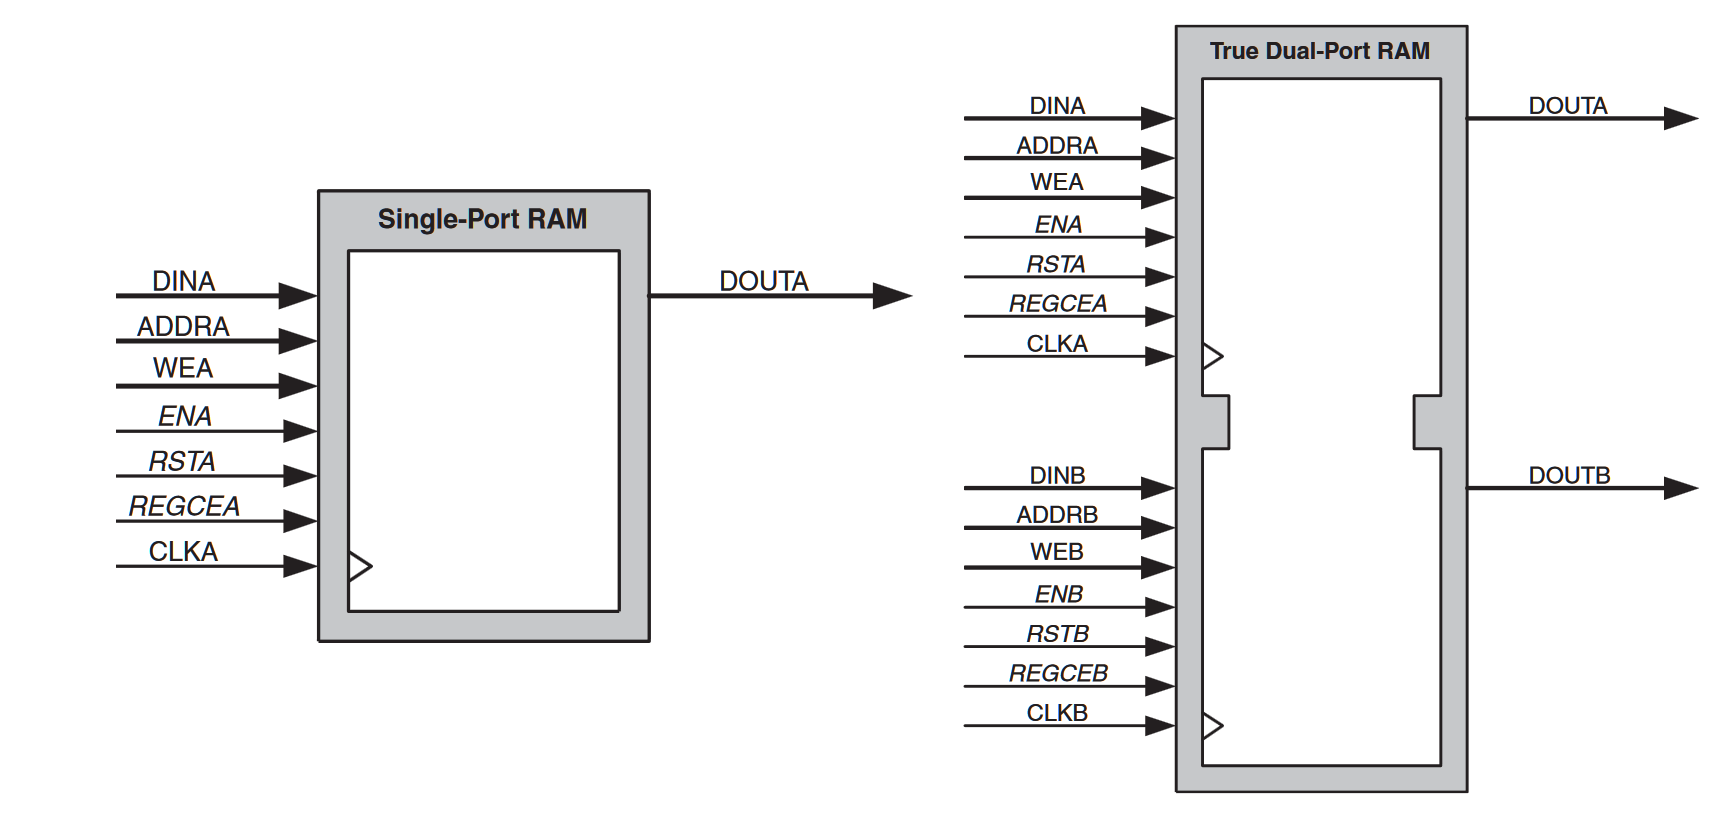
\includegraphics[width=12cm]{img/rams.png}
\caption{\label{fig:rams}Tipos de memorias RAM implementadas}
\end{center}
\end{figure}

Las memorias RAM de puerto doble (derecha en la figura \ref{fig:rams}) funcionan exactamente de la misma manera, salvo que poseen los puertos de entrada y salida duplicados. De esta forma se puede leer y escribir en el mismo instante, siempre que sea en direcciones diferentes. Este tipo de memorias serán adecuadas cuando la lectura y escritura no estén claramente distanciadas en el tiempo, por ejemplo, en el caso de la salida. Tras el procesado inverso de la iFFT, las muestras deben almacenarse en memoria de forma continua, sin interrupción, lo que podría causar problemas si justo en ese momento fuera necesario leer una muestra para escribirla en el búfer de salida.

Esto es la consecuencia de no realizar todas las operaciones bajo el mismo periodo de reloj: mientras que el muestreo se realiza a frecuencia $F_{s}=48,8kHz$, el reloj general del sistema tiene una frecuencia $F_{clk} = 100MHz$. La razón para realizar esta conversión es que si todo el sistema trabajase a la frecuencia de muestreo, las operaciones tardarían demasiado en realizarse, aumentando en gran medida la latencia. 

Ambos tipos de memorias poseen las mismas características, salvo que dependiendo del lugar que ocupen en la cadena de datos, el tamaño de la palabra y el número de direcciones que poseen varían. Estas memorias tienen un \emph{pipeline} interno que provoca un retraso en dos ciclos en la lectura, ciclos durante los cuales es necesario mantener la señal de \emph{enable} activa. La documentación que proporciona Xillinx y los ficheros auxiliares que se generan al sintetizar estos módulos facilitan el correcto tratamiento y configuración de los bloques de memorias.

\subsection{Core FFT e iFFT}
Análogamente al caso de las memorias, también se ha utilizado el módulo de Vivado para realizar las transformadas de Fourier.
\section{Controlador global}
h
\subsection{Displays}
h 